\documentclass[conference]{IEEEtran}

\usepackage[T1]{fontenc}
\usepackage[utf8]{inputenc}
\usepackage{pgfplots}
\pgfplotsset{compat=1.18}
\usepackage{tikz}
\usetikzlibrary{shapes.geometric, arrows.meta, positioning, calc}
\usepackage{booktabs}
\usepackage{array}
\usepackage{hyperref}
\usepackage{xcolor}
\usepackage{graphicx}
\usepackage{float}
\usepackage{enumitem}
\usepackage{amsmath}
\usepackage{balance}

\definecolor{ieeblue}{HTML}{1A5276}
\definecolor{accent}{HTML}{C0392B}
\definecolor{chartblue}{HTML}{2874A6}
\definecolor{chartgreen}{HTML}{1E8449}
\definecolor{chartorange}{HTML}{CA6F1E}
\definecolor{chartred}{HTML}{C0392B}
\definecolor{chartpurple}{HTML}{6C3483}
\definecolor{chartgray}{HTML}{5D6D7E}
\definecolor{chartteal}{HTML}{148F77}
\definecolor{inkcolor}{HTML}{0D0D0D}
\definecolor{papercolor}{HTML}{F2EFE9}
\definecolor{accentred}{HTML}{E8341A}

\hypersetup{
    colorlinks=true,
    linkcolor=ieeblue,
    urlcolor=ieeblue,
    citecolor=ieeblue
}

\begin{document}

\title{Idea Lab: A Self-Service Cross-Disciplinary\\Team Formation Platform for DBIT}

\author{
\IEEEauthorblockN{Harsha N\textsuperscript{1}, Mithun Gowda B\textsuperscript{2}, Naren V\textsuperscript{3}, Nevil Anson Dsouza\textsuperscript{4}}
\IEEEauthorblockA{Department of Computer Science and Engineering, Section B\\
Don Bosco Institute of Technology, Bangalore, India\\
\textsuperscript{1}harsha210108@gmail.com,
\textsuperscript{2}mithungowda.b7411@gmail.com\\
\textsuperscript{3}narenbhaskar2007@gmail.com,
\textsuperscript{4}nevilansondsouza@gmail.com}
}

\maketitle

% ============================================================
\begin{abstract}
% ============================================================
This paper presents \textbf{Idea Lab}, a web-based team formation platform developed for Don Bosco Institute of Technology (DBIT), Bangalore. The platform enables approximately 825 first-year students across 7 engineering branches to self-organize into cross-disciplinary teams of exactly 6 members with real-time constraint validation and administrative oversight. Built using Next.js 16, Firebase Firestore, and a custom OTP-based authentication system, Idea Lab replaces the manual team assignment process with an automated, constraint-enforced, and scalable solution. The system enforces branch diversity constraints, provides real-time notifications, and offers comprehensive admin controls for managing student registrations and team compositions. The platform is deployed at \url{https://idea-lab-sage.vercel.app/}.
\end{abstract}

\begin{IEEEkeywords}
Team Formation, Web Application, Next.js, Firebase, Cross-Disciplinary Teams, Real-Time Validation, OTP Authentication
\end{IEEEkeywords}

% ============================================================
\section{Introduction}
% ============================================================

Forming balanced, cross-disciplinary teams from a large student body is a recurring challenge in educational institutions. Manual assignment methods are time-consuming, error-prone, and often fail to account for branch diversity requirements. At Don Bosco Institute of Technology (DBIT), approximately 825 first-year students across 7 engineering branches---CSE, ISE, AIML, ECE, EEE, CV, and ME---need to form teams for interdisciplinary project work in the Idea Lab program.

\textbf{Idea Lab} addresses this challenge by providing a self-service platform where students can register, create teams, invite members, and join existing teams while the system automatically enforces composition constraints in real time.

The key contributions of this work are:
\begin{itemize}[noitemsep,topsep=3pt]
    \item A real-time team formation system with automated constraint validation
    \item A custom OTP-based authentication system using the Brevo Email API
    \item A comprehensive admin dashboard with gate controls and bulk data management
    \item A production-grade security architecture with JWT sessions, rate limiting, and Firestore security rules
\end{itemize}

\smallskip
\noindent\textbf{Repository:} \url{https://github.com/harshaxyZ/idea.lab.git}\\
\textbf{Live URL:} \url{https://idea-lab-sage.vercel.app/}

% ============================================================
\section{System Architecture}
% ============================================================

\subsection{High-Level Architecture}

Idea Lab follows a modern full-stack architecture with server-side rendering and API routes provided by Next.js~16 (App Router), backed by Firebase Firestore as the primary database.

\begin{figure}[htbp]
\centering
\resizebox{\columnwidth}{!}{%
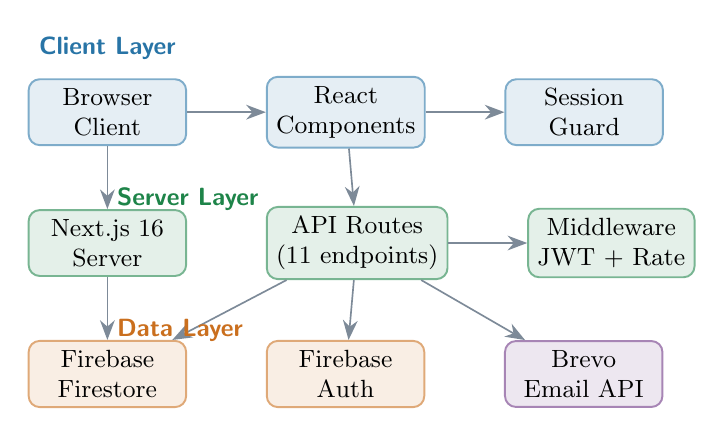
\begin{tikzpicture}[
    node distance=0.8cm and 1.0cm,
    every node/.style={font=\small},
    block/.style={draw, rounded corners=4pt, minimum width=2cm, minimum height=0.8cm, align=center, line width=0.7pt},
    client/.style={block, fill=chartblue!12, draw=chartblue!60},
    server/.style={block, fill=chartgreen!12, draw=chartgreen!60},
    db/.style={block, fill=chartorange!12, draw=chartorange!60},
    ext/.style={block, fill=chartpurple!12, draw=chartpurple!60},
    arrow/.style={-{Stealth[length=2.5mm]}, semithick, draw=chartgray!80},
    lbl/.style={font=\small\bfseries\sffamily}
]
    % Client Layer
    \node[client] (browser) {Browser\\Client};
    \node[client, right=of browser] (react) {React\\Components};
    \node[client, right=of react] (session) {Session\\Guard};

    % Server Layer
    \node[server, below=of browser] (nextjs) {Next.js 16\\Server};
    \node[server, right=of nextjs] (api) {API Routes\\(11 endpoints)};
    \node[server, right=of api] (mw) {Middleware\\JWT + Rate};

    % Data Layer
    \node[db, below=of nextjs] (firestore) {Firebase\\Firestore};
    \node[db, right=of firestore] (auth) {Firebase\\Auth};
    \node[ext, right=of auth] (brevo) {Brevo\\Email API};

    % Arrows
    \draw[arrow] (browser) -- (react);
    \draw[arrow] (react) -- (session);
    \draw[arrow] (browser) -- (nextjs);
    \draw[arrow] (react) -- (api);
    \draw[arrow] (api) -- (mw);
    \draw[arrow] (nextjs) -- (firestore);
    \draw[arrow] (api) -- (firestore);
    \draw[arrow] (api) -- (auth);
    \draw[arrow] (api) -- (brevo);

    % Layer labels
    \node[lbl, color=chartblue, above=0.12cm of browser] {Client Layer};
    \node[lbl, color=chartgreen, above=0.12cm of nextjs, anchor=west] {Server Layer};
    \node[lbl, color=chartorange, above=0.12cm of firestore, anchor=west] {Data Layer};
\end{tikzpicture}%
}
\caption{High-level system architecture of Idea Lab.}
\label{fig:architecture}
\end{figure}

\subsection{Firestore Data Model}

The system uses 8 Firestore collections as shown in Table~\ref{tab:collections}.

\begin{table}[htbp]
\centering
\caption{Firestore Collections and Their Purposes}
\label{tab:collections}
\footnotesize
\renewcommand{\arraystretch}{1.15}
\begin{tabular}{@{}ll@{}}
\toprule
\textbf{Collection} & \textbf{Purpose} \\
\midrule
\texttt{students} & CSV-imported master student data \\
\texttt{registrations} & Active registered students \\
\texttt{teams} & Team records with member lists \\
\texttt{invites} & Invite and join request documents \\
\texttt{notifications} & Real-time user notifications \\
\texttt{config} & Global configuration flags \\
\texttt{otp\_codes} & Email verification codes \\
\texttt{admins} & Admin whitelist entries \\
\bottomrule
\end{tabular}
\end{table}

% ============================================================
\section{Technology Stack}
% ============================================================

\begin{figure}[htbp]
\centering
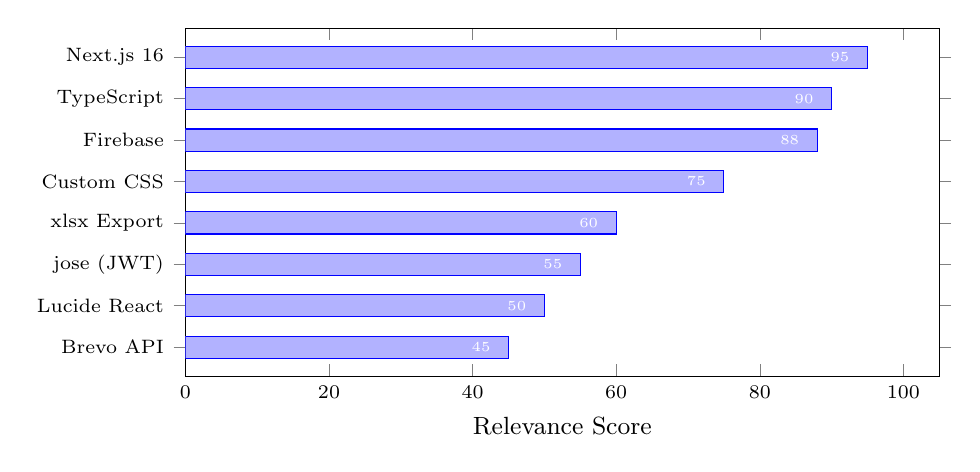
\begin{tikzpicture}
\begin{axis}[
    xbar,
    width=0.92\columnwidth,
    height=6cm,
    xlabel={\small Relevance Score},
    symbolic y coords={
        {Brevo API},
        {Lucide React},
        {jose (JWT)},
        {xlsx Export},
        {Custom CSS},
        {Firebase},
        {TypeScript},
        {Next.js 16}
    },
    ytick=data,
    y tick label style={font=\scriptsize},
    x tick label style={font=\scriptsize},
    xlabel style={font=\scriptsize},
    nodes near coords,
    nodes near coords style={font=\tiny\bfseries, color=white, anchor=east, xshift=-3pt},
    bar width=8pt,
    xmin=0, xmax=105,
    every axis plot/.append style={fill=chartblue!85, draw=chartblue},
    enlarge y limits=0.1,
]
\addplot coordinates {
    (95,{Next.js 16})
    (90,{TypeScript})
    (88,{Firebase})
    (75,{Custom CSS})
    (60,{xlsx Export})
    (55,{jose (JWT)})
    (50,{Lucide React})
    (45,{Brevo API})
};
\end{axis}
\end{tikzpicture}
\caption{Technology stack components ranked by relevance.}
\label{fig:techstack}
\end{figure}

Table~\ref{tab:techstack} provides a detailed breakdown.

\begin{table}[htbp]
\centering
\caption{Detailed Technology Stack}
\label{tab:techstack}
\footnotesize
\renewcommand{\arraystretch}{1.15}
\begin{tabular}{@{}p{1.4cm}p{5.4cm}@{}}
\toprule
\textbf{Layer} & \textbf{Technology} \\
\midrule
Framework & Next.js 16 (App Router, SSR) \\
Language & TypeScript 5 (strict mode) \\
Database & Firebase Firestore (NoSQL) \\
Auth & Firebase Auth (admin) + Custom OTP \\
Email & Brevo Email API (multi-key round-robin) \\
Styling & Custom CSS (Paper \& Ink design system) \\
Session & JWT (HS256, httpOnly cookie) \\
Export & xlsx library for Excel generation \\
Icons & Lucide React \\
Hosting & Vercel (serverless deployment) \\
\bottomrule
\end{tabular}
\end{table}

% ============================================================
\section{Key Features}
% ============================================================

\subsection{Student Registration Flow}

The registration process follows a three-step flow:

\begin{enumerate}[noitemsep,topsep=3pt]
    \item \textbf{USN Entry} --- validated against CSV master data via \texttt{/api/auth/lookup-usn}
    \item \textbf{OTP Verification} --- 6-digit code sent via Brevo Email API with 10-minute expiry, rate-limited to 5 sends per 15 minutes per IP
    \item \textbf{Session Establishment} --- JWT cookie + Firebase custom token issued for dual authentication
\end{enumerate}

\subsection{Team Formation with Constraint Enforcement}

Teams must satisfy the constraints shown in Table~\ref{tab:constraints}.

\begin{table}[htbp]
\centering
\caption{Team Composition Constraints}
\label{tab:constraints}
\footnotesize
\renewcommand{\arraystretch}{1.15}
\begin{tabular}{@{}lll@{}}
\toprule
\textbf{Rule} & \textbf{Value} & \textbf{Enforcement} \\
\midrule
Team size & Exactly 6 & Hard block at 6 \\
Max same branch & 4 from one & Blocked at 5th \\
Min branches & 2 unique & Checked at completion \\
EEE/ECE req. & At least 1 & Warning $\to$ hard block \\
\bottomrule
\end{tabular}
\end{table}

\subsection{Admin Dashboard}

The admin panel provides six functional tabs: (1)~\textbf{Dashboard} with real-time statistics, (2)~\textbf{Students} for CSV upload with batch writes of 450 documents per batch, (3)~\textbf{Registrations} with searchable, paginated tables supporting CSV/XLS export, (4)~\textbf{Teams} for filtered team views, (5)~\textbf{Admins} for whitelist management, and (6)~\textbf{Settings} for gate controls and database reset.

% ============================================================
\section{Codebase Analysis}
% ============================================================

\subsection{Project Statistics}

The project comprises \textbf{58 TypeScript/TSX files} totaling \textbf{10,937 lines of code}.

\begin{figure}[htbp]
\centering
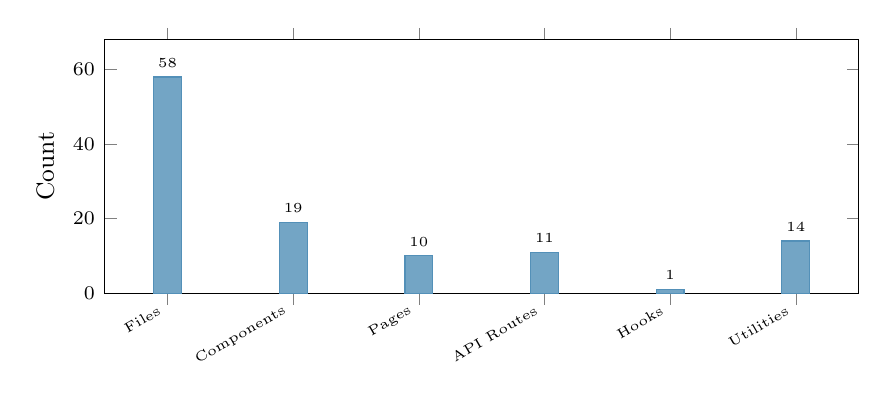
\begin{tikzpicture}
\begin{axis}[
    ybar,
    width=0.92\columnwidth,
    height=4.8cm,
    ylabel={\small Count},
    ylabel style={font=\scriptsize},
    symbolic x coords={Files, Components, Pages, API Routes, Hooks, Utilities},
    xtick=data,
    x tick label style={font=\tiny, rotate=30, anchor=east},
    y tick label style={font=\scriptsize},
    nodes near coords,
    nodes near coords style={font=\tiny\bfseries},
    bar width=10pt,
    ymin=0, ymax=68,
    enlarge x limits=0.1,
    every axis plot/.append style={draw=chartblue!80},
]
\addplot[fill=chartblue!65] coordinates {
    (Files, 58)
    (Components, 19)
    (Pages, 10)
    (API Routes, 11)
    (Hooks, 1)
    (Utilities, 14)
};
\end{axis}
\end{tikzpicture}
\caption{Codebase composition by category.}
\label{fig:codebase}
\end{figure}

\subsection{Source File Distribution}

\begin{figure}[htbp]
\centering
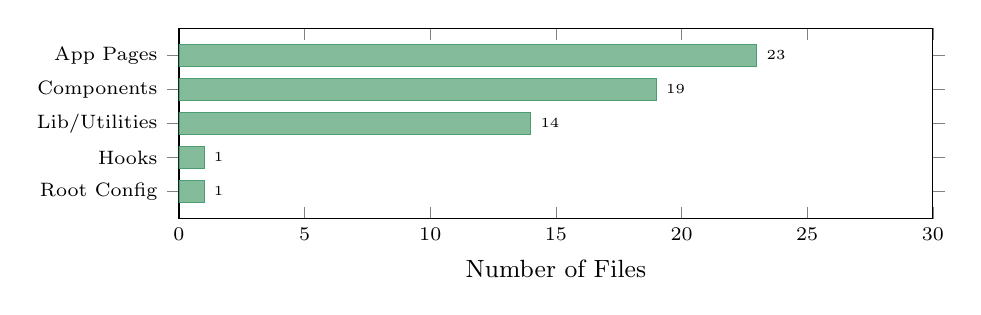
\begin{tikzpicture}
\begin{axis}[
    xbar,
    width=0.92\columnwidth,
    height=4cm,
    xlabel={\small Number of Files},
    xlabel style={font=\scriptsize},
    symbolic y coords={
        {Root Config},
        {Hooks},
        {Lib/Utilities},
        {Components},
        {App Pages}
    },
    ytick=data,
    y tick label style={font=\scriptsize},
    x tick label style={font=\scriptsize},
    nodes near coords,
    nodes near coords style={font=\tiny\bfseries},
    bar width=8pt,
    xmin=0, xmax=30,
    enlarge y limits=0.2,
    every axis plot/.append style={draw=chartgreen!80},
]
\addplot[fill=chartgreen!55] coordinates {(23,{App Pages}) (19,{Components}) (14,{Lib/Utilities}) (1,{Hooks}) (1,{Root Config})};
\end{axis}
\end{tikzpicture}
\caption{Source file distribution by directory.}
\label{fig:distribution}
\end{figure}

\subsection{File Type Breakdown}

The codebase contains \textbf{31 TSX} files (React components and pages) and \textbf{29 TS} files (logic, utilities, API routes, and configuration).

\begin{figure}[htbp]
\centering
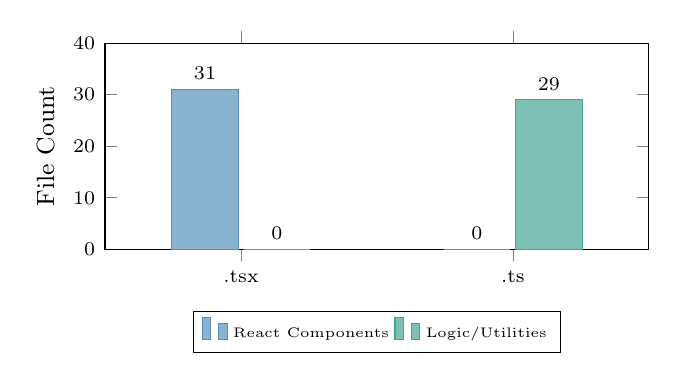
\begin{tikzpicture}
\begin{axis}[
    ybar,
    width=0.7\columnwidth,
    height=4.2cm,
    ylabel={\small File Count},
    ylabel style={font=\scriptsize},
    symbolic x coords={.tsx, .ts},
    xtick=data,
    x tick label style={font=\scriptsize},
    y tick label style={font=\scriptsize},
    bar width=24pt,
    ymin=0, ymax=40,
    nodes near coords,
    nodes near coords style={font=\scriptsize\bfseries},
    legend style={at={(0.5,-0.3)}, anchor=north, font=\tiny, legend columns=2},
    enlarge x limits=0.5,
]
\addplot[fill=chartblue!55, draw=chartblue!80] coordinates {(.tsx, 31) (.ts, 0)};
\addplot[fill=chartteal!55, draw=chartteal!80] coordinates {(.tsx, 0) (.ts, 29)};
\legend{React Components, Logic/Utilities}
\end{axis}
\end{tikzpicture}
\caption{TypeScript file type distribution.}
\label{fig:filetypes}
\end{figure}

% ============================================================
\section{Development Timeline}
% ============================================================

The project was developed over a 5-day sprint from March 11--15, 2026, producing \textbf{62 commits}.

\begin{figure}[htbp]
\centering
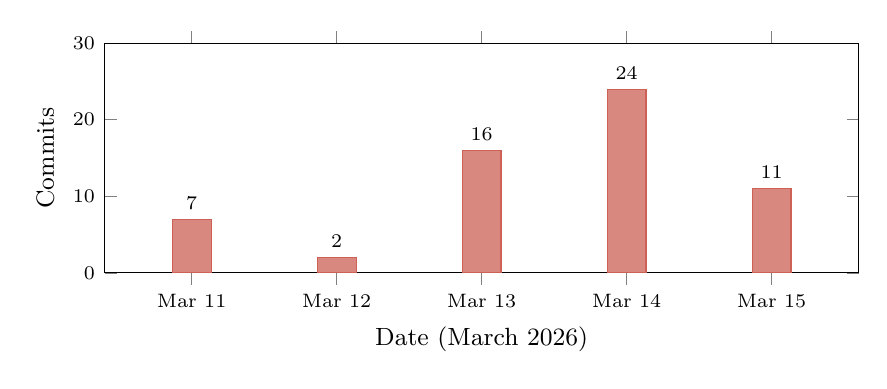
\begin{tikzpicture}
\begin{axis}[
    ybar,
    width=0.92\columnwidth,
    height=4.5cm,
    ylabel={\small Commits},
    ylabel style={font=\scriptsize},
    xlabel={\small Date (March 2026)},
    xlabel style={font=\scriptsize},
    symbolic x coords={Mar 11, Mar 12, Mar 13, Mar 14, Mar 15},
    xtick=data,
    x tick label style={font=\scriptsize},
    y tick label style={font=\scriptsize},
    nodes near coords,
    nodes near coords style={font=\scriptsize\bfseries},
    bar width=14pt,
    ymin=0, ymax=30,
    enlarge x limits=0.15,
    every axis plot/.append style={draw=accent!80},
]
\addplot[fill=accent!60] coordinates {
    (Mar 11, 7)
    (Mar 12, 2)
    (Mar 13, 16)
    (Mar 14, 24)
    (Mar 15, 11)
};
\end{axis}
\end{tikzpicture}
\caption{Commit activity during the development sprint.}
\label{fig:timeline}
\end{figure}

\subsection{Contribution Distribution}

\begin{figure}[htbp]
\centering
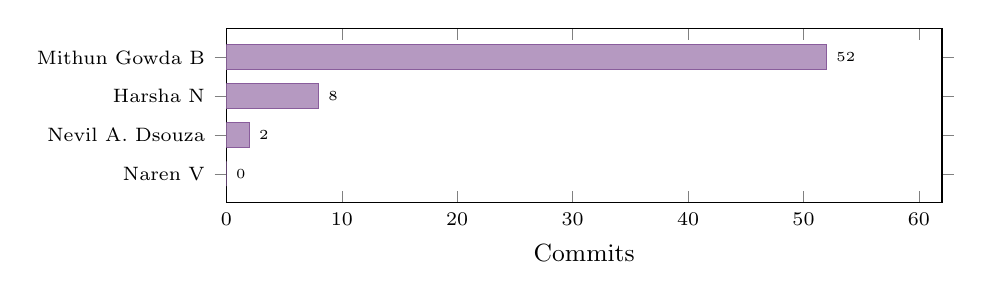
\begin{tikzpicture}
\begin{axis}[
    xbar,
    width=0.88\columnwidth,
    height=3.8cm,
    xlabel={\small Commits},
    xlabel style={font=\scriptsize},
    symbolic y coords={
        {Naren V},
        {Nevil A. Dsouza},
        {Harsha N},
        {Mithun Gowda B}
    },
    ytick=data,
    y tick label style={font=\scriptsize},
    x tick label style={font=\scriptsize},
    nodes near coords,
    nodes near coords style={font=\tiny\bfseries},
    bar width=9pt,
    xmin=0, xmax=62,
    enlarge y limits=0.25,
    every axis plot/.append style={draw=chartpurple!80},
]
\addplot[fill=chartpurple!50] coordinates {(52,{Mithun Gowda B}) (8,{Harsha N}) (2,{Nevil A. Dsouza}) (0,{Naren V})};
\end{axis}
\end{tikzpicture}
\caption{Team contribution distribution by commits.}
\label{fig:contributions}
\end{figure}

% ============================================================
\section{Security Architecture}
% ============================================================

\subsection{Authentication Layers}

The system implements a multi-layered authentication approach as illustrated in Fig.~\ref{fig:security}.

\begin{figure}[htbp]
\centering
\resizebox{0.95\columnwidth}{!}{%
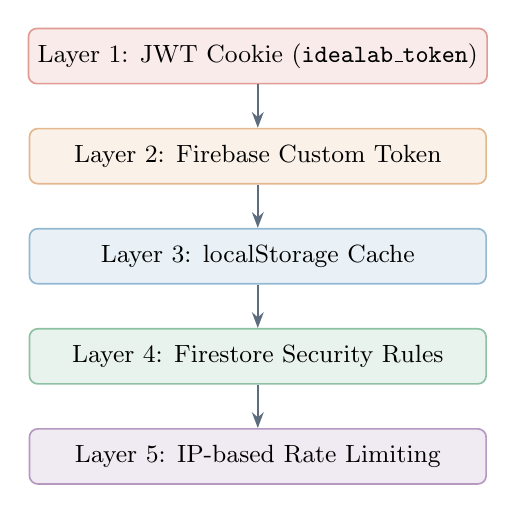
\begin{tikzpicture}[
    node distance=0.55cm,
    every node/.style={font=\small},
    layer/.style={draw, rounded corners=3pt, minimum width=5.8cm, minimum height=0.7cm, align=center, line width=0.6pt}
]
    \node[layer, fill=chartred!10, draw=chartred!50] (l1) {Layer 1: JWT Cookie (\texttt{idealab\_token})};
    \node[layer, fill=chartorange!10, draw=chartorange!50, below=of l1] (l2) {Layer 2: Firebase Custom Token};
    \node[layer, fill=chartblue!10, draw=chartblue!50, below=of l2] (l3) {Layer 3: localStorage Cache};
    \node[layer, fill=chartgreen!10, draw=chartgreen!50, below=of l3] (l4) {Layer 4: Firestore Security Rules};
    \node[layer, fill=chartpurple!10, draw=chartpurple!50, below=of l4] (l5) {Layer 5: IP-based Rate Limiting};

    \draw[-{Stealth[length=2mm]}, semithick, chartgray] (l1) -- (l2);
    \draw[-{Stealth[length=2mm]}, semithick, chartgray] (l2) -- (l3);
    \draw[-{Stealth[length=2mm]}, semithick, chartgray] (l3) -- (l4);
    \draw[-{Stealth[length=2mm]}, semithick, chartgray] (l4) -- (l5);
\end{tikzpicture}%
}
\caption{Multi-layered security architecture.}
\label{fig:security}
\end{figure}

\subsection{Rate Limiting}

\begin{table}[htbp]
\centering
\caption{API Rate Limiting Configuration}
\label{tab:ratelimit}
\footnotesize
\renewcommand{\arraystretch}{1.15}
\begin{tabular}{@{}lll@{}}
\toprule
\textbf{Endpoint} & \textbf{Limit} & \textbf{Window} \\
\midrule
\texttt{POST send-otp} & 5 req/IP & 15 min \\
\texttt{POST verify-otp} & 10 att/IP & 15 min \\
Per-OTP attempts & 5 attempts & Until expiry \\
Per-email cooldown & 1 OTP & 60 sec \\
\bottomrule
\end{tabular}
\end{table}

\subsection{Security Headers}

The application enforces security headers via Next.js middleware: \texttt{X-Frame-Options: DENY}, \texttt{X-Content-Type-Options: nosniff}, \texttt{Strict-Transport-Security} (HSTS), \texttt{Content-Security-Policy} (CSP), and \texttt{Permissions-Policy} (camera, microphone, and geolocation disabled).

% ============================================================
\section{User Flow Analysis}
% ============================================================

\begin{figure}[htbp]
\centering
\resizebox{0.95\columnwidth}{!}{%
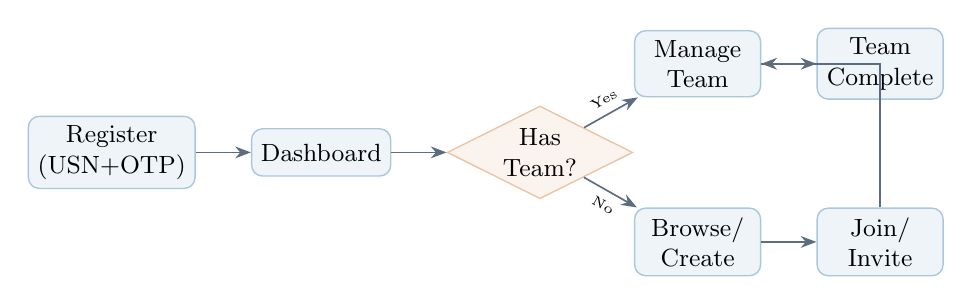
\begin{tikzpicture}[
    node distance=0.5cm and 0.7cm,
    every node/.style={font=\small},
    flowstep/.style={draw, rounded corners=4pt, minimum width=1.6cm, minimum height=0.6cm, align=center, fill=chartblue!8, draw=chartblue!40, line width=0.5pt},
    decision/.style={draw, diamond, aspect=2, minimum width=1.2cm, align=center, fill=chartorange!8, draw=chartorange!40, line width=0.5pt, inner sep=1pt, font=\small},
    arrow/.style={-{Stealth[length=2mm]}, draw=chartgray, semithick}
]
    \node[flowstep] (reg) {Register\\(USN+OTP)};
    \node[flowstep, right=of reg] (dash) {Dashboard};
    \node[decision, right=of dash] (has) {Has\\Team?};
    \node[flowstep, above right=0.4cm and 0.6cm of has] (manage) {Manage\\Team};
    \node[flowstep, below right=0.4cm and 0.6cm of has] (find) {Browse/\\Create};
    \node[flowstep, right=of find] (join) {Join/\\Invite};
    \node[flowstep, right=of manage] (done) {Team\\Complete};

    \draw[arrow] (reg) -- (dash);
    \draw[arrow] (dash) -- (has);
    \draw[arrow] (has) -- node[above, sloped, font=\tiny] {Yes} (manage);
    \draw[arrow] (has) -- node[below, sloped, font=\tiny] {No} (find);
    \draw[arrow] (find) -- (join);
    \draw[arrow] (join) |- (manage);
    \draw[arrow] (manage) -- (done);
\end{tikzpicture}%
}
\caption{Student user flow through the platform.}
\label{fig:userflow}
\end{figure}

% ============================================================
\section{Team Details}
% ============================================================

\begin{table}[htbp]
\centering
\caption{Project Team Members}
\label{tab:team}
\footnotesize
\renewcommand{\arraystretch}{1.25}
\begin{tabular}{@{}clll@{}}
\toprule
\textbf{\#} & \textbf{Name} & \textbf{USN} & \textbf{Email} \\
\midrule
1 & Harsha N & 1DB25CS065 & harsha210108 \\
2 & Mithun Gowda B & 1DB25CS109 & mithungowda.b7411 \\
3 & Naren V & 1DB25CS113 & narenbhaskar2007 \\
4 & Nevil Anson Dsouza & 1DB25CS116 & nevilansondsouza \\
\bottomrule
\multicolumn{4}{@{}l}{\scriptsize All emails use the @gmail.com domain.}
\end{tabular}
\end{table}

\begin{table}[htbp]
\centering
\caption{Team Member Contact Details}
\label{tab:teamroles}
\footnotesize
\renewcommand{\arraystretch}{1.25}
\begin{tabular}{@{}llll@{}}
\toprule
\textbf{Name} & \textbf{Phone} & \textbf{Branch} & \textbf{Sec.} \\
\midrule
Harsha N & 7899214458 & CSE & B \\
Mithun Gowda B & 9844556496 & CSE & B \\
Naren V & 7204375655 & CSE & B \\
Nevil Anson Dsouza & 9980445460 & CSE & B \\
\bottomrule
\end{tabular}
\end{table}

\noindent All team members are first-year B.E.\ students in the \textbf{Department of Computer Science and Engineering~(CSE), Section~B} at \textbf{Don Bosco Institute of Technology~(DBIT)}, Bangalore, affiliated to Visvesvaraya Technological University~(VTU).

\subsection{Individual Contributions}

\begin{itemize}[noitemsep,topsep=3pt]
    \item \textbf{Mithun Gowda B} --- Lead developer. Implemented the core architecture, authentication system (JWT~+ OTP), team constraint engine, admin dashboard, API routes, middleware, security layers, and deployment. Authored 52 of 62 commits~(84\%).
    \item \textbf{Harsha N} --- Contributed to the Brevo OTP authentication integration, invite system enhancements, and pull request workflows. Authored 8 commits~(13\%).
    \item \textbf{Nevil Anson Dsouza} --- Contributed to admin panel functionality and server-side API route migrations. Authored 2 commits~(3\%).
    \item \textbf{Naren V} --- Participated in code review, testing, and quality assurance throughout the development cycle.
\end{itemize}

% ============================================================
\section{Deployment \& Infrastructure}
% ============================================================

\begin{table}[htbp]
\centering
\caption{Deployment Configuration}
\label{tab:deploy}
\footnotesize
\renewcommand{\arraystretch}{1.15}
\begin{tabular}{@{}ll@{}}
\toprule
\textbf{Component} & \textbf{Details} \\
\midrule
Hosting & Vercel (serverless) \\
Database & Firebase Firestore (Google Cloud) \\
Email & Brevo API (300 emails/day free tier) \\
Domain & idea-lab-sage.vercel.app \\
Repository & github.com/harshaxyZ/idea.lab \\
Build & Next.js 16 \\
CI/CD & Vercel Git Integration (auto-deploy) \\
\bottomrule
\end{tabular}
\end{table}

% ============================================================
\section{Design System}
% ============================================================

The platform uses a custom design system called ``Paper~\& Ink'' with a minimal, print-inspired aesthetic built on four core colors:

\begin{figure}[htbp]
\centering
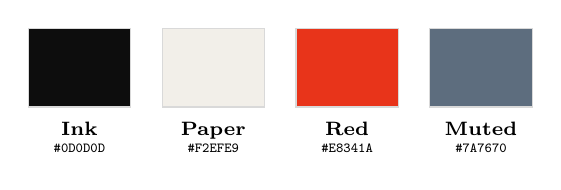
\begin{tikzpicture}
    % Ink
    \fill[inkcolor] (0, 0) rectangle ++(1.3, 1);
    \draw[gray!30] (0, 0) rectangle ++(1.3, 1);
    \node[font=\scriptsize\bfseries, below=2pt] at (0.65, 0) {Ink};
    \node[font=\tiny, below=10pt] at (0.65, 0) {\texttt{\#0D0D0D}};
    % Paper
    \fill[papercolor] (1.7, 0) rectangle ++(1.3, 1);
    \draw[gray!30] (1.7, 0) rectangle ++(1.3, 1);
    \node[font=\scriptsize\bfseries, below=2pt] at (2.35, 0) {Paper};
    \node[font=\tiny, below=10pt] at (2.35, 0) {\texttt{\#F2EFE9}};
    % Red
    \fill[accentred] (3.4, 0) rectangle ++(1.3, 1);
    \draw[gray!30] (3.4, 0) rectangle ++(1.3, 1);
    \node[font=\scriptsize\bfseries, below=2pt] at (4.05, 0) {Red};
    \node[font=\tiny, below=10pt] at (4.05, 0) {\texttt{\#E8341A}};
    % Muted
    \fill[chartgray] (5.1, 0) rectangle ++(1.3, 1);
    \draw[gray!30] (5.1, 0) rectangle ++(1.3, 1);
    \node[font=\scriptsize\bfseries, below=2pt] at (5.75, 0) {Muted};
    \node[font=\tiny, below=10pt] at (5.75, 0) {\texttt{\#7A7670}};
\end{tikzpicture}
\caption{Paper \& Ink design system color palette.}
\label{fig:colors}
\end{figure}

% ============================================================
\section{Challenges \& Solutions}
% ============================================================

\begin{table}[htbp]
\centering
\caption{Key Challenges and Solutions}
\label{tab:challenges}
\footnotesize
\renewcommand{\arraystretch}{1.15}
\begin{tabular}{@{}p{3.1cm}p{3.6cm}@{}}
\toprule
\textbf{Challenge} & \textbf{Solution} \\
\midrule
Email rate limits (300/day) & Multi-key round-robin rotation \\
Race conditions in team joins & Firestore transactions + server-side validation \\
SSR hydration mismatches & SessionGuard with client-only rendering \\
Cross-origin API abuse & Origin-checking middleware \\
Large CSV uploads & Batch writes (450 docs/batch) \\
\bottomrule
\end{tabular}
\end{table}

% ============================================================
\section{Future Work}
% ============================================================

\begin{itemize}[noitemsep,topsep=3pt]
    \item Integration with university ERP systems for automatic student data synchronization
    \item Real-time collaborative team workspace with shared documents
    \item AI-powered team recommendation engine based on student skills and interests
    \item Mobile application for improved accessibility
    \item Analytics dashboard with team performance metrics
\end{itemize}

% ============================================================
\section{Conclusion}
% ============================================================

Idea Lab demonstrates that a self-service, constraint-enforced team formation platform can effectively replace manual processes at scale. The system handles 825+ students across 7 branches with real-time validation, ensuring every team meets diversity requirements. The 5-day development sprint produced a production-grade application with 10,937 lines of TypeScript, 19 reusable components, 11 API routes, and comprehensive security layers. The platform is deployed at \url{https://idea-lab-sage.vercel.app/}, with source code at \url{https://github.com/harshaxyZ/idea.lab.git}.

\balance
\begin{thebibliography}{9}
\bibitem{nextjs} Vercel, ``Next.js Documentation,'' 2026. [Online]. Available: \url{https://nextjs.org/docs}
\bibitem{firebase} Google, ``Firebase Documentation,'' 2026. [Online]. Available: \url{https://firebase.google.com/docs}
\bibitem{brevo} Brevo, ``Email API Documentation,'' 2026. [Online]. Available: \url{https://developers.brevo.com}
\bibitem{jwt} IETF, ``RFC 7519 --- JSON Web Token (JWT),'' May 2015.
\bibitem{owasp} OWASP Foundation, ``OWASP Top Ten Web Application Security Risks,'' 2021. [Online]. Available: \url{https://owasp.org/www-project-top-ten/}
\bibitem{firestore} Google, ``Cloud Firestore Security Rules,'' 2026. [Online]. Available: \url{https://firebase.google.com/docs/firestore/security/get-started}
\end{thebibliography}

\end{document}
